\section{Utilisasi Sumber Daya Akselerator}

Pada subbab \ref{sec:fpga}, metrik utilisasi sumber daya terdiri atas 3 hal:

\begin{enumerate}
	\item \acf{LUTs}\\
	      \ac{LUTs} adalah blok dasar dari logika yang digunakan dalam \ac{FPGA}. Metrik penggunaan \ac{LUTs} mengindikasikan seberapa banyak sumber daya logika yang digunakan oleh desain pada \ac{FPGA}. Semakin tinggi penggunaan \ac{LUTs}, semakin kompleks dan padat logika yang diimplementasikan.
	\item \textit{Flip-flops}\\
	      \textit{Flip-flops} adalah elemen penyimpanan dasar dalam \ac{FPGA} yang digunakan untuk menyimpan bit data. Penggunaan \textit{flip-flops} mencerminkan kebutuhan desain terhadap penyimpanan data sementara dan kemampuan untuk menangani operasi sekuensial.
	\item \textit{Block \ac{RAM}}\\
	      \textit{Block \ac{RAM}} adalah memori terintegrasi dalam \ac{FPGA} yang digunakan untuk menyimpan data dalam jumlah besar. Metrik penggunaan \textit{block \ac{RAM}} memberikan gambaran tentang kebutuhan desain terhadap memori, termasuk berapa banyak data yang perlu disimpan dan diakses secara cepat selama operasi.
\end{enumerate}

Berikut, pada Gambar \ref{fig:plot-resource}, merupakan hasil utilisasi sumber daya akselerator dari sintesis desain \textit{processor} VeeR EL2 tanpa dan dengan implementasi akselerator.

\begin{figure}[h]
	\centering
	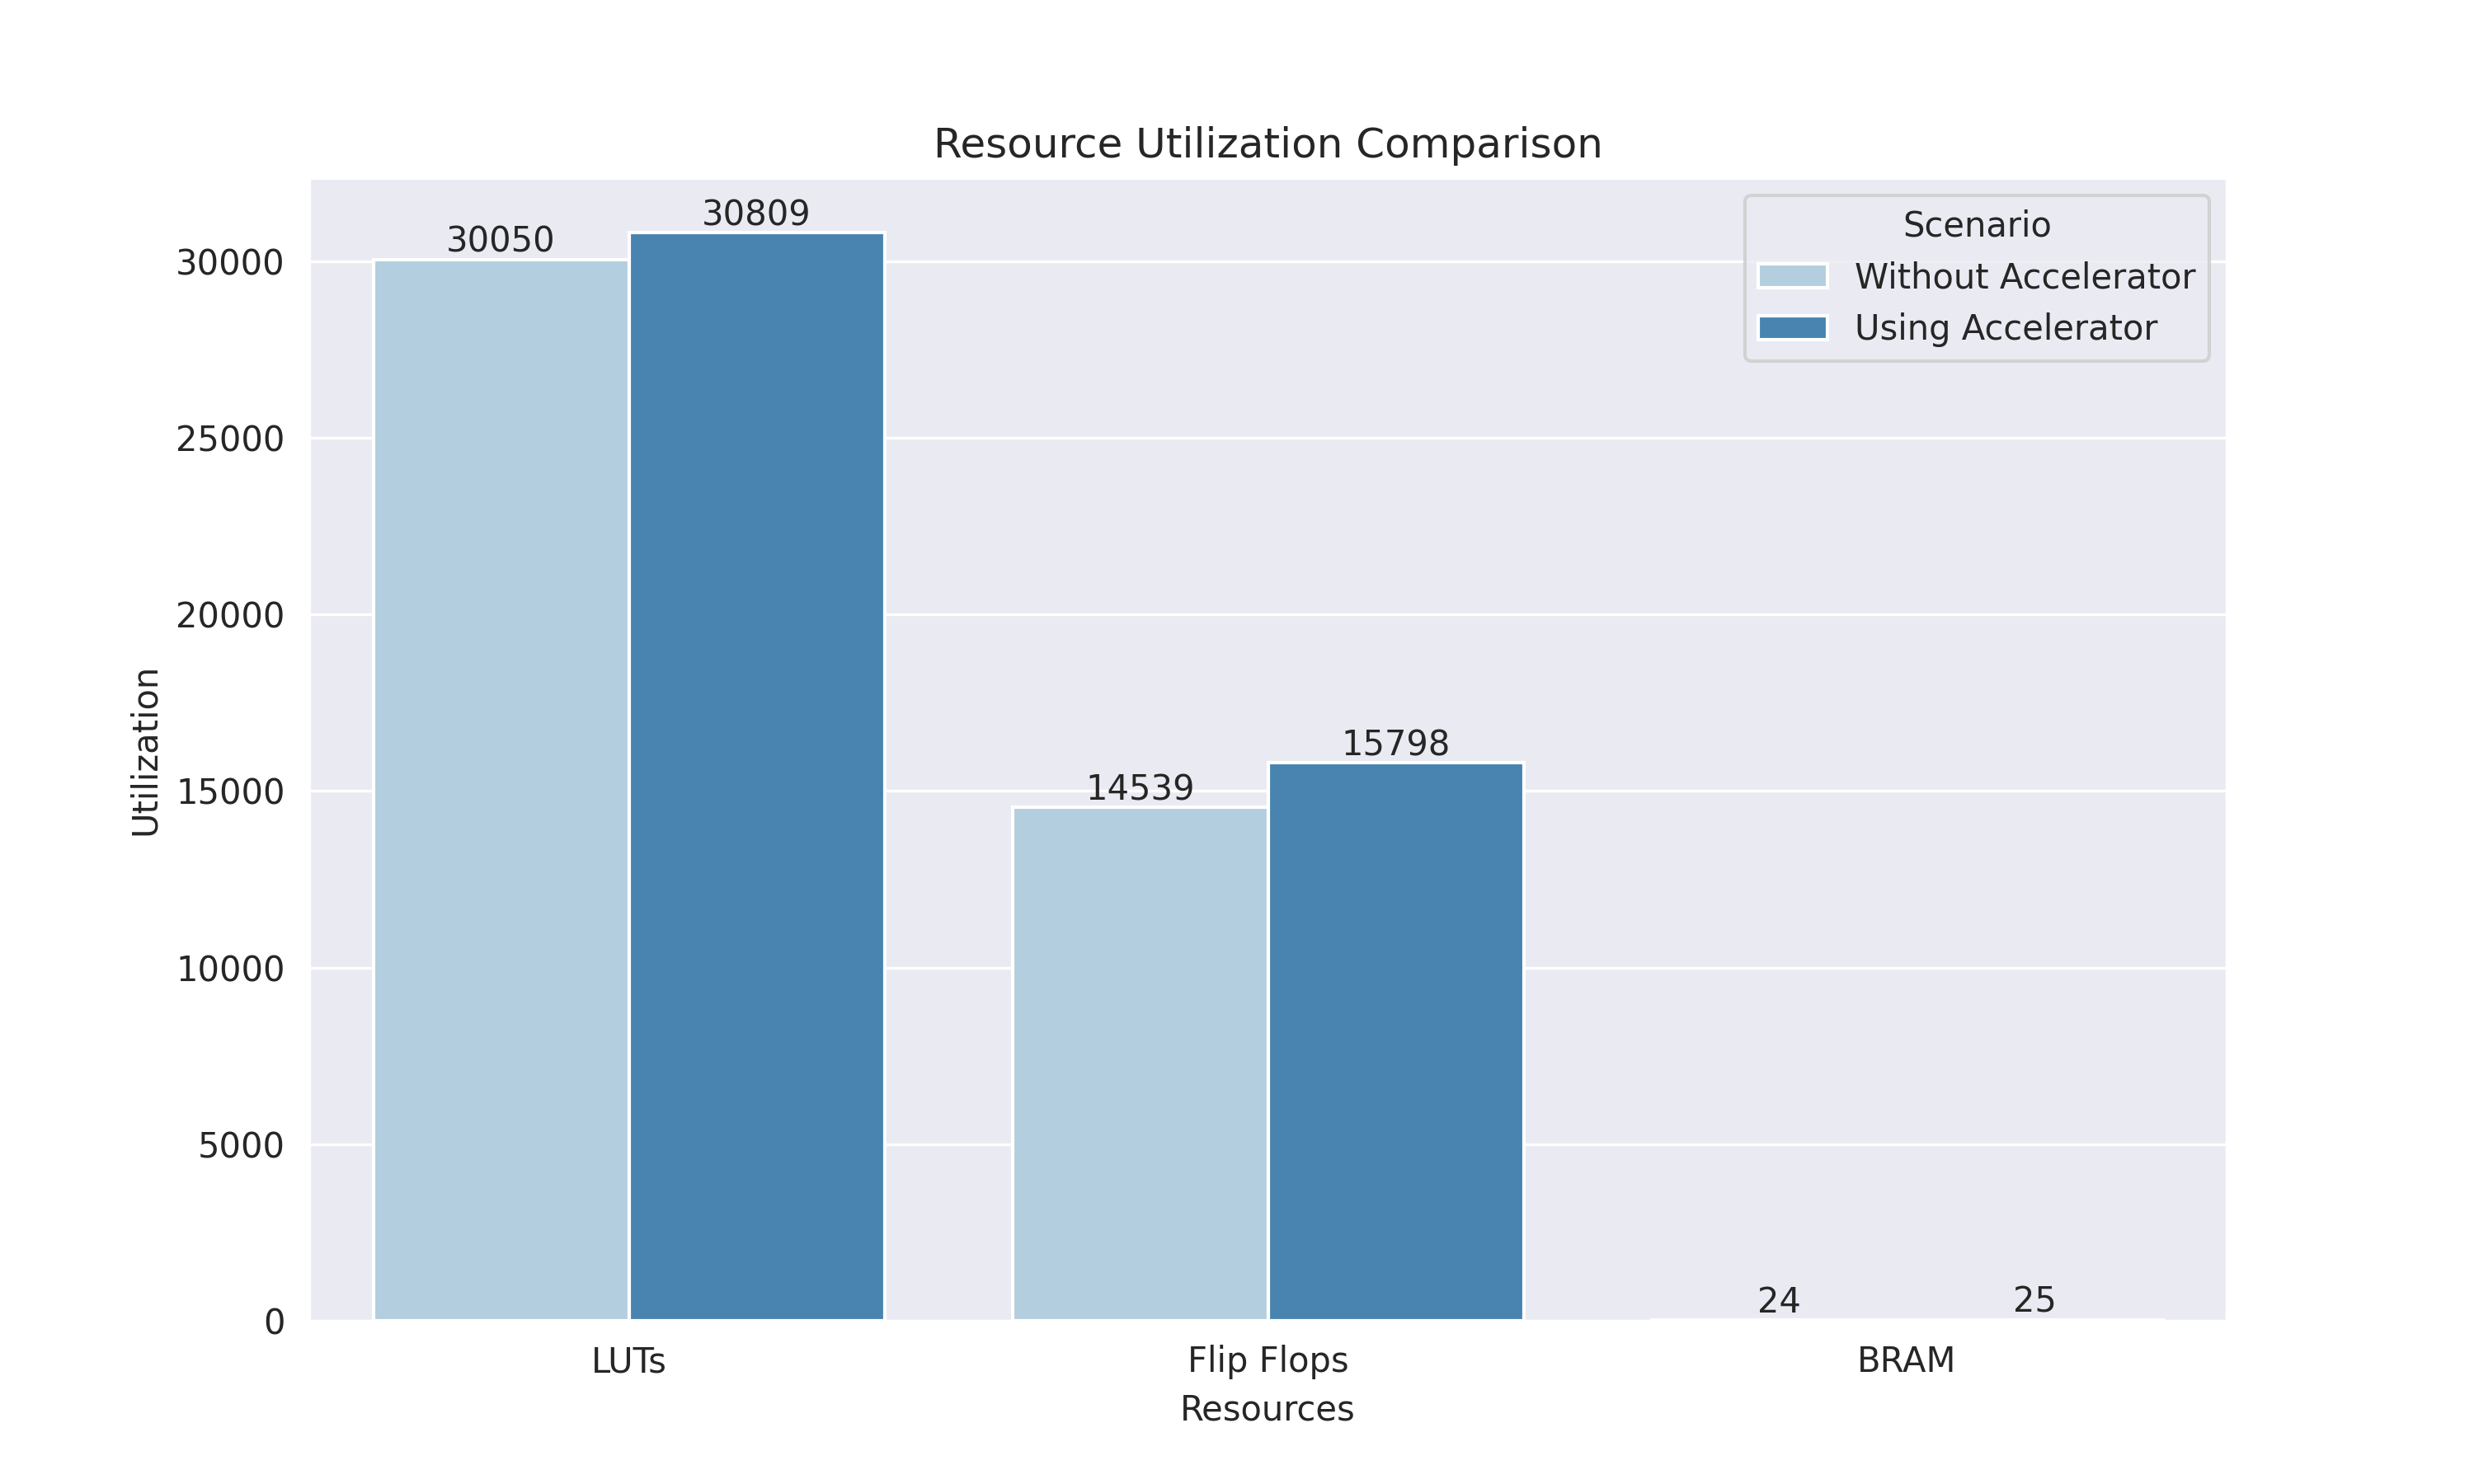
\includegraphics[width=1\textwidth]{chapter-4/plot-resource.png}
	\caption{Plot hasil penggunaan sumber daya pada \ac{FPGA}}
	\label{fig:plot-resource}
\end{figure}

Dapat diperhatikan pada Gambar \ref{fig:plot-resource}, perubahan banyaknya penggunaan \ac{LUTs}, \textit{flip-flops}, dan \textit{block \ac{RAM}} itu relatif sedikit. Lebih jelasnya lagi, Gambar \ref{fig:plot-resource-increase} mendeskripsikan tentang kenaikan persentase penggunaan sumber daya tersebut beserta dengan banyaknya sumber daya yang masih tersisa pada \ac{FPGA}.

\begin{figure}[h]
	\centering
	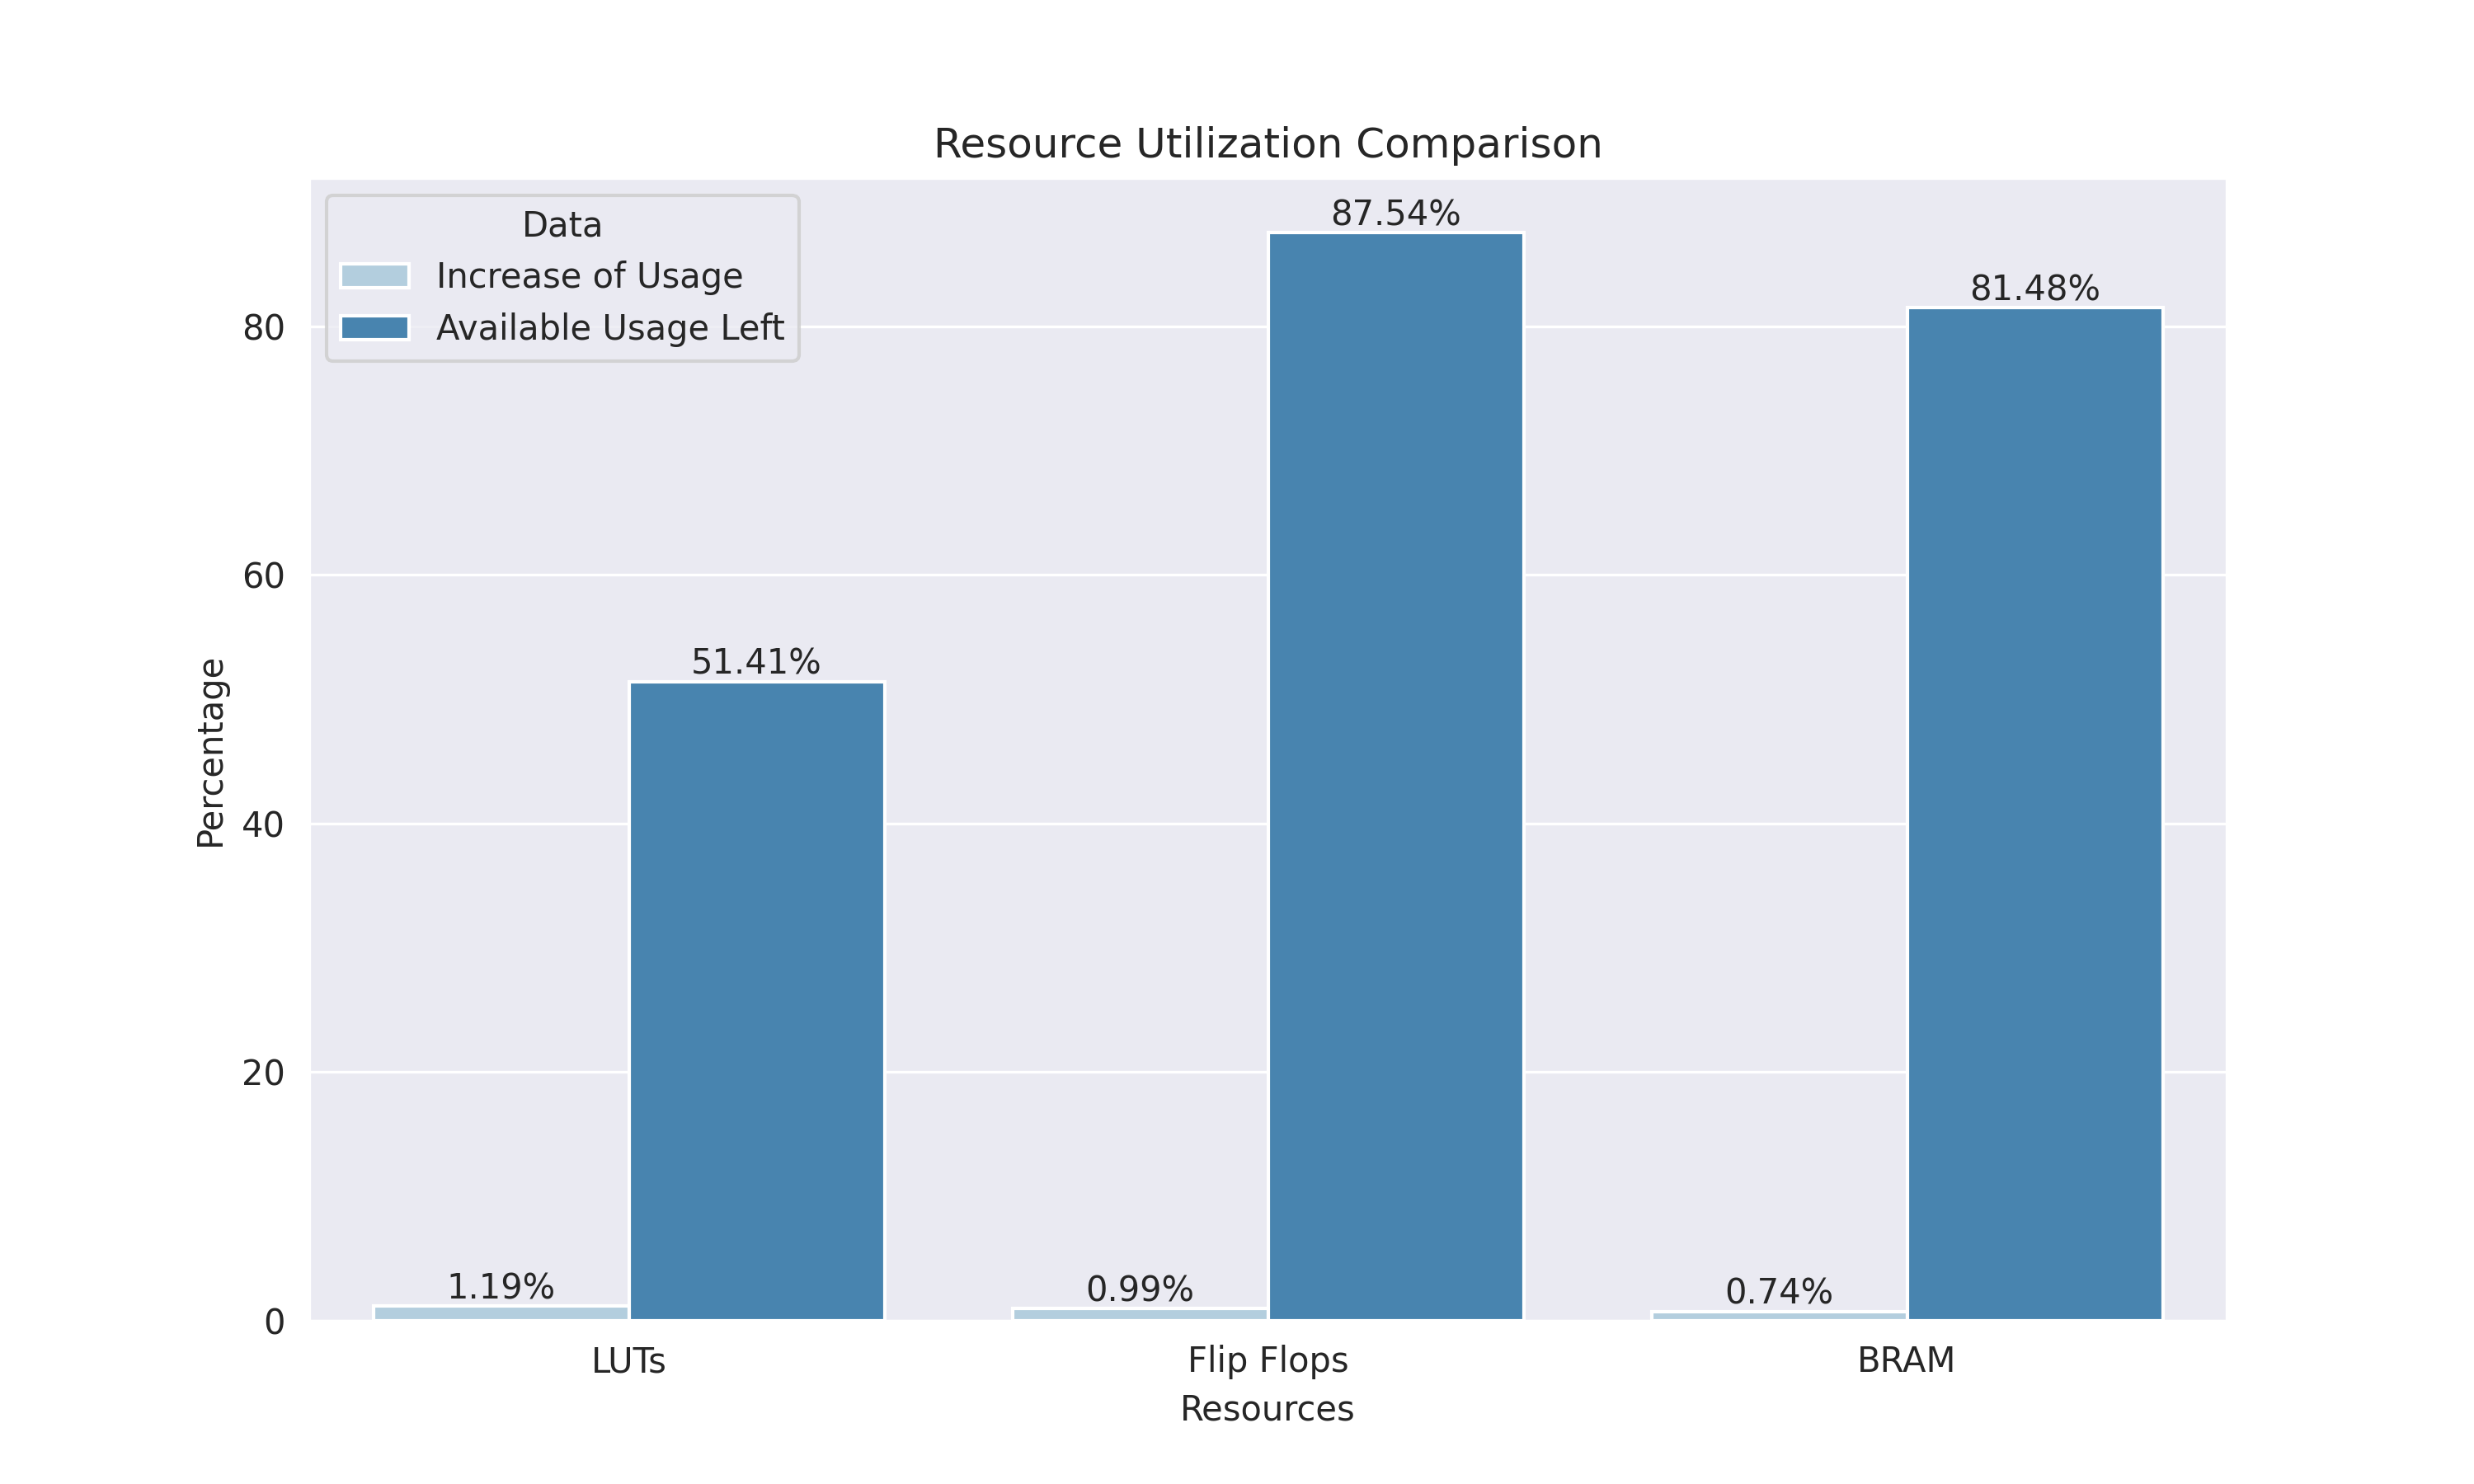
\includegraphics[width=1\textwidth]{chapter-4/plot-resource-increase.png}
	\caption{Plot penambahan penggunaan sumber daya pada \ac{FPGA}}
	\label{fig:plot-resource-increase}
\end{figure}

Seluruh peningkatan sumber daya masih berada dibawah 1.5\% dengan sisa sumber daya tersedia yang masih sangatlah banyak, berarti implementasi akselerator perangkat keras berhasil dibangun secara efisien. Selanjutnya, bila dibandingkan dengan implementasi akselerator-akselerator penelitian sebelumnya yang terdapat pada subbab \ref{sec:accelerator-researches} maka didapatkan data sesuai dengan Tabel \ref{tab:comparison-utilization}.


\begin{table}[h]
	\centering
	\caption{Perbandingan utilisasi sumber daya dengan akselerator riset sebelumnya}
	\label{tab:comparison-utilization}
	\renewcommand{\arraystretch}{1.2}
	\setlength{\tabcolsep}{3pt}
	\begin{tabularx}{\textwidth}{|p{20mm}|X|X|X|X|X|X|X|}
		\hline
		\textbf{Reference}            & \multicolumn{2}{c|}{Spanò et al. \parencite{spano2019efficient}} & Da Silva et al. \parencite{dasilva2019parallel} & Y. Meng et al. \parencite{meng2020generic} & \multicolumn{2}{c|}{Sutisna et al. \parencite{sutisna2023faraneq}} & Proposed                            \\ \hline
		\textbf{Design Level}         & \multicolumn{4}{c|}{Standalone Core}                             & \multicolumn{3}{c|}{System on Chip}                                                                                                                                                                     \\ \hline
		\textbf{Action Policy}        & \multicolumn{2}{c|}{NA}                                          & random                                          & $\epsilon$-greedy                          & \multicolumn{2}{c|}{decreasing-$\epsilon$}                         & $\epsilon$-greedy                   \\ \hline
		\textbf{Number of Agents (G)} & single                                                           & single                                          & single                                     & double                                                             & single            & single & single \\ \hline
		\textbf{Bit Width}            & 16                                                               & 32                                              & 30                                         & 16                                                                 & 16                & 32     & 32     \\ \hline
		\textbf{LUT}                  & 333                                                              & 682                                             & 77574                                      & 172                                                                & 2490              & 2062   & 759    \\ \hline
		\textbf{Registers}            & 258                                                              & 606                                             & 13175                                      & NA                                                                 & 2348              & 2179   & 1259   \\ \hline
		\textbf{BRAM}                 & NA                                                               & NA                                              & 266                                        & NA                                                                 & 22                & 20     & 1      \\ \hline
	\end{tabularx}
\end{table}

Pada tabel \ref{tab:comparison-utilization}, dapat diperhatikan bahwa implementasi akselerator yang dibangun pada riset ini merupakan akselerator yang terefisien kedua pada ukuran 32-bit. Hal ini, menunjukkan kemungkinan penggunaan akselerator pada tahap produksi karena dapat bersaing dengan \textit{state of the art} dari penelitian terkini.
